\documentclass[14pt, a4paper]{extarticle}

\usepackage[margin=1in]{geometry}
\usepackage{graphicx}
\usepackage{enumitem}
\usepackage{multicol}
\usepackage{fancyhdr}
\usepackage{amsfonts}
\usepackage{amssymb}
\usepackage{listings}
\usepackage{float}
\usepackage{wrapfig}

\usepackage{gvv-book}
\usepackage{gvv}

\graphicspath{ {figs/} }

\pagestyle{fancy}
\fancyhf{} 
\fancyhead[L]{2013}
\fancyhead[R]{PH}
\fancyfoot[L]{PH}
\fancyfoot[R]{\thepage/15}
\renewcommand{\headrulewidth}{0.4pt}
\renewcommand{\footrulewidth}{0.4pt}

\let\oldvec\vec
\renewcommand{\vec}[1]{\overrightarrow{#1}}
\newcommand{\myvec}[1]{\begin{bmatrix} #1 \end{bmatrix}}

\begin{document}

\textbf{Q. 1 -- Q. 25 carry one mark each.}

\begin{enumerate}[label=\textbf{Q. \arabic*}]

\item $f(x)$ is a symmetric periodic function of x i.e. $f(x) = f(-x)$. Then, in general, the Fourier series of the function $f(x)$ will be of the form
\begin{enumerate}
        \item $ f(x) = \sum_{n=1}^{\infty} (a_n \cos(nkx) + b_n \sin(nkx)) $
        \item $ f(x) = a_0 + \sum_{n=1}^{\infty} (a_n \cos(nkx)) $
        \item $ f(x) = \sum_{n=1}^{\infty} (b_n \sin(nkx)) $
        \item $ f(x) = a_0 + \sum_{n=1}^{\infty} (b_n \sin(nkx)) $
    \end{enumerate}
    \hfill \textbf{(GATE PH 2013)}

\item In the most general case, which one of the following quantities is NOT a second order tensor?
\begin{multicols}{2}
    \begin{enumerate}
        \item Stress
        \item Strain
        \item Moment of inertia
        \item Pressure
    \end{enumerate}
\end{multicols}
\hfill \textbf{(GATE PH 2013)}

\item An electron is moving with a velocity of $0.85c$ in the same direction as that of a moving photon. The relative velocity of the electron with respect to photon is
\begin{multicols}{4}
    \begin{enumerate}
        \item $c$
        \item $-c$
        \item $0.15c$
        \item $-0.15c$
    \end{enumerate}
\end{multicols}
\hfill \textbf{(GATE PH 2013)}

 \item If Planck's constant were zero, then the total energy contained in a box filled with radiation of all frequencies at temperature $T$ would be ( $k$ is the Boltzmann constant and $T$ is nonzero)
    \begin{multicols}{4}
        \begin{enumerate}
            \item Zero
            \item Infinite
            \item $\frac{3}{2}kT$
            \item $kT$
        \end{enumerate}
    \end{multicols}
    \hfill \textbf{(GATE PH 2013)}

\item Across a first order phase transition, the free energy is    
    \begin{enumerate}
        \item proportional to the temperature
        \item a discontinuous function of the temperature
        \item a continuous function of the temperature but its first derivative is discontinuous
        \item such that the first derivative with respect to temperature is continuous
    \end{enumerate}
    \hfill \textbf{(GATE PH 2013)}

\item Two gases separated by an impermeable but movable partition are allowed to freely exchange energy. At equilibrium, the two sides will have the same    
    \begin{enumerate}
        \item pressure and temperature
        \item volume and temperature
        \item pressure and volume
        \item volume and energy
    \end{enumerate}
    \hfill \textbf{(GATE PH 2013)}

\item The entropy function of a system is given by $S(E) = a E (E_0 - E)$ where $a$ and $E_0$ are positive constants. The temperature of the system is
\begin{enumerate}
    \item negative for some energies
    \item increases monotonically with energy
    \item decreases monotonically with energy
    \item Zero
\end{enumerate}
\hfill \textbf{(GATE PH 2013)}

\item Consider a linear collection of $N$ independent spin $1/2$ particles, each at a fixed location. The entropy of this system is ($k$ is the Boltzmann constant)
\begin{multicols}{4}
    \begin{enumerate}
        \item Zero
        \item $Nk$
        \item $\frac{1}{2}Nk$
        \item $Nk \ln(2)$
    \end{enumerate}
\end{multicols}
\hfill \textbf{(GATE PH 2013)}

\item The decay process $n \to p^+ + e^- + \bar{\nu}_e$ violates
\begin{multicols}{2}
    \begin{enumerate}
        \item baryon number
        \item lepton number
        \item isospin
        \item strangeness
    \end{enumerate}
\end{multicols}
\hfill \textbf{(GATE PH 2013)}

\item The isospin ($I$) and baryon number ($B$) of the up quark is
\begin{multicols}{2}
    \begin{enumerate}
        \item $I=1, B=1$
        \item $I=1, B=1/3$
        \item $I=1/2, B=1$
        \item $I=1/2, B=1/3$
    \end{enumerate}
\end{multicols}
\hfill \textbf{(GATE PH 2013)}

\item Consider the scattering of neutrons by protons at very low energy due to a nuclear potential of range $r_0$. Given that,
\begin{align*}
    \cot(kr_0 + \delta) \approx -\frac{\gamma}{k}
\end{align*}
where $\delta$ is the phase shift, $k$ the wave number and $(-\gamma)$ the logarithmic derivative of the deuteron ground state wave function, the phase shift is
\begin{multicols}{4}
    \begin{enumerate}
        \item $\delta \approx -\frac{k}{\gamma} kr_0$
        \item $\delta \approx -\frac{\gamma}{k} kr_0$
        \item $\delta \approx \frac{\pi}{2} - kr_0$
        \item $\delta \approx -\frac{\pi}{2} - kr_0$
    \end{enumerate}
\end{multicols}
\hfill \textbf{(GATE PH 2013)}

\item In the $\beta$ decay process, the transition $2^+ \to 3^+$, is
\begin{enumerate}
    \item allowed both by Fermi and Gamow-Teller selection rule
    \item allowed by Fermi and but not by Gamow-Teller selection rule
    \item not allowed by Fermi but allowed by Gamow-Teller selection rule
    \item not allowed both by Fermi and Gamow-Teller selection rule
\end{enumerate}
\hfill \textbf{(GATE PH 2013)}

\item At a surface current, which one of the magnetostatic boundary condition is NOT CORRECT?
\begin{enumerate}
    \item Normal component of the magnetic field is continuous.
    \item Normal component of the magnetic vector potential is continuous.
    \item Tangential component of the magnetic vector potential is continuous.
    \item Tangential component of the magnetic vector potential is not continuous.
\end{enumerate}
\hfill \textbf{(GATE PH 2013)}

\item Interference fringes are seen at an observation plane $z = 0$, by the superposition of two plane waves $A_1\exp[i(\vec{k}_1 \cdot \vec{r} - \omega t)]$ and $A_2\exp[i(\vec{k}_2 \cdot \vec{r} - \omega t)]$, where $A_1$ and $A_2$ are real amplitudes. The condition for interference maximum is
\begin{enumerate}
    \item $(\vec{k}_1 - \vec{k}_2) \cdot \vec{r} = (2m+1)\pi$
    \item $(\vec{k}_1 - \vec{k}_2) \cdot \vec{r} = 2m\pi$
    \item $(\vec{k}_1 + \vec{k}_2) \cdot \vec{r} = (2m+1)\pi$
    \item $(\vec{k}_1 + \vec{k}_2) \cdot \vec{r} = 2m\pi$
\end{enumerate}
\hfill \textbf{(GATE PH 2013)}

\item For a scalar function $\varphi$ satisfying the Laplace equation, $\nabla\varphi$ has
\begin{enumerate}
    \item zero curl and non-zero divergence
    \item non-zero curl and zero divergence
    \item zero curl and zero divergence
    \item non-zero curl and non-zero divergence
\end{enumerate}
\hfill \textbf{(GATE PH 2013)}

\item A circularly polarized monochromatic plane wave is incident on a dielectric interface at Brewster angle. Which one of the following statements is CORRECT ?
\begin{enumerate}
    \item The reflected light is plane polarized in the plane of incidence and the transmitted light is circularly polarized.
    \item The reflected light is plane polarized perpendicular to the plane of incidence and the transmitted light is plane polarized in the plane of incidence.
    \item The reflected light is plane polarized perpendicular to the plane of incidence and the transmitted light is elliptically polarized.
    \item There will be no reflected light and the transmitted light is circularly polarized.
\end{enumerate}
\hfill \textbf{(GATE PH 2013)}

\item Which one of the following commutation relations is NOT CORRECT ? Here, symbols have their usual meanings.
\begin{enumerate}
    \item $[L^2, L_z] = 0$
    \item $[L_x, L_y] = i\hbar L_z$
    \item $[L_z, L_+] = \hbar L_+$
    \item $[L_z, L_-] = -\hbar L_-$
\end{enumerate}
\hfill \textbf{(GATE PH 2013)}

\item The Lagrangian of a system with one degree of freedom $q$ is given by $L = \alpha \dot{q}^2 + \beta q^2$, where $\alpha$ and $\beta$ are non-zero constants. If $p_q$ denotes the canonical momentum conjugate to $q$ then which one of the following statements is CORRECT?
\begin{enumerate}
    \item $p_q = 2\beta q$ and it is a conserved quantity.
    \item $p_q = 2\beta q$ and it is not a conserved quantity.
    \item $p_q = 2\alpha\dot{q}$ and it is a conserved quantity.
    \item $p_q = 2\alpha\dot{q}$ and it is not a conserved quantity.
\end{enumerate}
\hfill \textbf{(GATE PH 2013)}

\item What should be the clock frequency of a 6-bit A/D converter so that its maximum conversion time is $32\,\mu\text{s}$?
\begin{multicols}{4}
    \begin{enumerate}
        \item $1\,\text{MHz}$
        \item $2\,\text{MHz}$
        \item $0.5\,\text{MHz}$
        \item $4\,\text{MHz}$
    \end{enumerate}
\end{multicols}
\hfill \textbf{(GATE PH 2013)}

\item A phosphorous doped silicon semiconductor ( doping density: $10^{17}/\text{cm}^3$) is heated from $100^\circ\text{C}$ to $200^\circ\text{C}$. Which one of the following statements is CORRECT ?
\begin{enumerate}
    \item Position of Fermi level moves towards conduction band
    \item Position of dopant level moves towards conduction band
    \item Position of Fermi level moves towards middle of energy gap
    \item Position of dopant level moves towards middle of energy gap
\end{enumerate}
\hfill \textbf{(GATE PH 2013)}

\item Considering the BCS theory of superconductors, which one of the following statements is NOT CORRECT? ($h$ is the Planck's constant and $e$ is the electronic charge)
\begin{enumerate}
    \item Presence of energy gap at temperatures below the critical temperature
    \item Different critical temperatures for isotopes
    \item Quantization of magnetic flux in superconducting ring in the unit of ($h/e$)
    \item Presence of Meissner effect
\end{enumerate}
\hfill \textbf{(GATE PH 2013)}

\item Group I contains elementary excitations in solids. Group II gives the associated fields with these excitations. MATCH the excitations with their associated field and select your answer as per codes given below.
\begin{center}
    \begin{multicols}{2}
        \textbf{Group I}
        \begin{itemize}
            \item[(P)] phonon
            \item[(Q)] plasmon
            \item[(R)] polaron
            \item[(S)] polariton
        \end{itemize}
        \textbf{Group II}
        \begin{itemize}
            \item[(i)] photon + lattice vibration
            \item[(ii)] electron + elastic deformation
            \item[(iii)] collective electron oscillations
            \item[(iv)] elastic wave
        \end{itemize}
    \end{multicols}
\end{center}
Codes
\begin{enumerate}
    \item (P-iv), (Q-iii), (R-i), (S-ii)
    \item (P-iv), (Q-iii), (R-ii), (S-i)
    \item (P-i), (Q-iii), (R-ii), (S-iv)
    \item (P-iii), (Q-iv), (R-ii), (S-i)
\end{enumerate}
\hfill \textbf{(GATE PH 2013)}

\item The number of distinct ways of placing four indistinguishable balls into five distinguishable boxes is \underline{\hspace{5em}}.
\hfill \textbf{(GATE PH 2013)}

\item A voltage regulator has ripple rejection of $-50\,\text{dB}$. If input ripple is $1\,\text{mV}$, what is the output ripple voltage in $\mu\text{V}$? The answer should be up to two decimal places. \underline{\hspace{5em}}.
\hfill \textbf{(GATE PH 2013)}

\item The number of spectral lines allowed in the spectrum for the $3\,^2\text{D} \to 3\,^2\text{P}$ transition in sodium is \underline{\hspace{5em}}.
\textbf{(GATE PH 2013)}

\vspace{1.5em}

\textbf{Q. 26 to Q. 55 carry two marks each.}

\item Which of the following pairs of the given function $F(t)$ and its Laplace transform $f(s)$ is NOT CORRECT?
\begin{enumerate}
    \item $F(t) = \delta(t),~f(s)=1,$ (Singularity at +0)
    \item $F(t) = 1,~f(s) = \frac{1}{s},~(s>0)$
    \item $F(t) = \sin kt,~f(s) = \frac{k}{s^2+k^2},~(s>0)$
    \item $F(t) = te^{kt},~f(s) = \frac{1}{(s-k)^2},~(s>k, s>0)$
\end{enumerate}

\item If $\vec{A}$ and $\vec{B}$ are constant vectors, then $\nabla(\vec{A} \cdot \vec{B} \times \vec{r})$ is
\begin{multicols}{4}
    \begin{enumerate}
        \item $\vec{A} \cdot \vec{B}$
        \item $\vec{A} \times \vec{B}$
        \item $\vec{r}$
        \item Zero
    \end{enumerate}
\end{multicols}

\item $I(n + 1/2)$ is equal to [Given $\Gamma(n+1) = n\Gamma(n)$ and $\Gamma(1/2) = \sqrt{\pi}$]
\begin{multicols}{4}
    \begin{enumerate}
        \item $\frac{n!}{2n}\sqrt{\pi}$
        \item $\frac{(2n)!}{n!\,2^{2n}}\sqrt{\pi}$
        \item $\frac{2n!}{n!\,2^{2n}}\sqrt{\pi}$
        \item $\frac{n!}{2^{2n}}\sqrt{\pi}$
    \end{enumerate}
\end{multicols}

\item The relativistic form of Newton's second law of motion is
\begin{enumerate}
    \item $F = \frac{mc}{\sqrt{c^2-v^2}}\frac{dv}{dt}$
    \item $F = \frac{m\sqrt{c^2-v^2}}{c^2}\frac{dv}{dt}$
    \item $F = \frac{mc^2}{c^2-v^2}\frac{dv}{dt}$
    \item $F = m\frac{c^2}{c^2-v^2}\frac{dv}{dt}$
\end{enumerate}

\item Consider a gas of atoms obeying Maxwell-Boltzmann statistics. The average value of $e^{i\vec{a} \cdot \vec{p}}$ over all the momenta $\vec{p}$ of each of the particles (where $\vec{a}$ is a constant vector and $a$ is its magnitude, $m$ is the mass of each atom, $T$ is temperature and $k$ is Boltzmann's constant) is
\begin{multicols}{4}
    \begin{enumerate}
        \item One
        \item Zero
        \item $e^{-\frac{1}{2}a^2mkT}$
        \item $e^{-\frac{3}{2}a^2mkT}$
    \end{enumerate}
\end{multicols}
\hfill \textbf{(GATE PH 2013)}

\item The electromagnetic form factor $F(q^2)$ of a nucleus is given by,
\begin{align*}
 F(q^2) = \exp\left[-\frac{q^2}{2Q^2}\right]
\end{align*}
where $Q$ is a constant. Given that,
\begin{align*}
    F(q^2) &= \frac{4\pi}{q}\int_0^\infty rdr\,\rho(r)\sin qr \\
    \int d^3r\,\rho(r) &= 1
\end{align*}
where $\rho(r)$ is the charge density, the root mean square radius of the nucleus is given by,
\begin{multicols}{4}
    \begin{enumerate}
        \item $1/Q$
        \item $\sqrt{2}/Q$
        \item $\sqrt{3}/Q$
        \item $\sqrt{6}/Q$
    \end{enumerate}
\end{multicols}
\hfill \textbf{(GATE PH 2013)}

\item A uniform circular disk of radius $R$ and mass $M$ is rotating with angular speed $\omega$ about an axis, passing through its center and inclined at an angle $60^\circ$ with respect to its symmetry axis. The magnitude of the angular momentum of the disk is,
\begin{multicols}{4}
    \begin{enumerate}
        \item $\frac{\sqrt{5}}{4}\omega MR^2$
        \item $\frac{\sqrt{3}}{8}\omega MR^2$
        \item $\frac{\sqrt{7}}{8}\omega MR^2$
        \item $\frac{\sqrt{7}}{4}\omega MR^2$
    \end{enumerate}
\end{multicols}
\hfill \textbf{(GATE PH 2013)}

\item Consider two small blocks, each of mass $M$, attached to two identical springs. One of the springs is attached to the wall, as shown in the figure. The spring constant of each spring is $k$. The masses slide along the surface and the friction is negligible. The frequency of one of the normal modes of the system is,
\begin{figure}[H]
\centering
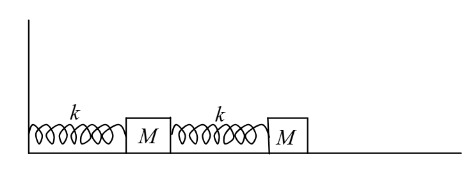
\includegraphics[width=0.5\textwidth]{figs/q.33fig2013.png}
\caption{two small blocks, each of mass M, attached to two identical
springs }
\label{fig:q33}
\end{figure}
\begin{enumerate}
\begin{multicols}{4}
\item $\frac{3+\sqrt{2}}{2}\sqrt{\frac{k}{M}}$
\item $\frac{\sqrt{3+\sqrt{3}}}{2}\sqrt{\frac{k}{M}}$
\item $\sqrt{\frac{3+\sqrt{5}}{2}}\sqrt{\frac{k}{M}}$
\item $\frac{\sqrt{3+\sqrt{6}}}{2}\sqrt{\frac{k}{M}}$
\end{multicols}
\end{enumerate}

\item A charge distribution has the charge density given by $\rho = Q\{\delta(x - x_0) - \delta(x + x_0)\}$. For this charge distribution the electric field at $(2x_0, 0,0)$
\begin{multicols}{4}
    \begin{enumerate}
        \item $\frac{2Q}{9\pi\epsilon_0x_0^2}$
        \item $\frac{Q}{4\pi\epsilon_0x_0^3}$
        \item $\frac{Q}{4\pi\epsilon_0x_0^2}$
        \item $\frac{Q}{16\pi\epsilon_0x_0^2}$
    \end{enumerate}
\end{multicols}
\hfill \textbf{(GATE PH 2013)}

\item A monochromatic plane wave at oblique incidence undergoes reflection at a dielectric interface. If $\hat{k}_i$, $\hat{k}_r$ and $\hat{n}$ are the unit vectors in the directions of incident wave, reflected wave and the normal to the surface respectively, which one of the following expressions is correct?
\begin{multicols}{2}
    \begin{enumerate}
        \item $(\hat{k}_i - \hat{k}_r) \times \hat{n} \ne 0$
        \item $(\hat{k}_i - \hat{k}_r) \cdot \hat{n} = 0$
        \item $(\hat{k}_i \times \hat{n}) \cdot \hat{k}_r = 0$
        \item $(\hat{k}_i \times \hat{n}) \cdot \hat{k}_r \ne 0$
    \end{enumerate}
\end{multicols}
\hfill \textbf{(GATE PH 2013)}

\item In a normal Zeeman effect experiment, spectral splitting of the line at the wavelength $643.8\,\text{nm}$ corresponding to the transition $5\,^1\text{D}_2 \to 5\,^1\text{P}_1$ of cadmium atoms is to be observed. The spectrometer has a resolution of $0.01\,\text{nm}$. The minimum magnetic field needed to observe this is ($m_e = 9.1 \times 10^{-31}\,\text{kg}$, $e = 1.6 \times 10^{-19}\,\text{C}$, $c = 3 \times 10^8\,\text{m/s}$)
\begin{multicols}{4}
    \begin{enumerate}
        \item $0.26\,\text{T}$
        \item $0.52\,\text{T}$
        \item $2.6\,\text{T}$
        \item $5.2\,\text{T}$
    \end{enumerate}
\end{multicols}
\hfill \textbf{(GATE PH 2013)}

\item The spacing between vibrational energy levels in CO molecule is found to be $8.44 \times 10^{-2}\,\text{eV}$. Given that the reduced mass of CO is $1.14 \times 10^{-26}\,\text{kg}$, Planck's constant is $6.626 \times 10^{-34}\,\text{Js}$ and $1\,\text{eV} = 1.6 \times 10^{-19}\,\text{J}$. The force constant of the bond in CO molecule is
\begin{multicols}{4}
    \begin{enumerate}
        \item $1.87\,\text{N/m}$
        \item $18.7\,\text{N/m}$
        \item $187\,\text{N/m}$
        \item $1870\,\text{N/m}$
    \end{enumerate}
\end{multicols}
\hfill \textbf{(GATE PH 2013)}

\item A lattice has the following primitive vectors (in $\r{A}$): $\vec{a} = 2(\hat{j} + \hat{k})$, $\vec{b} = 2(\hat{k} + \hat{i})$, $\vec{c} = 2(\hat{i} + \hat{j})$. The reciprocal lattice corresponding to the above lattice is
\begin{enumerate}
    \item BCC lattice with cube edge of $(\pi/2)\,\r{A}^{-1}$
    \item BCC lattice with cube edge of $(2\pi)\,\r{A}^{-1}$
    \item FCC lattice with cube edge of $(\pi/2)\,\r{A}^{-1}$
    \item FCC lattice with cube edge of $(2\pi)\,\r{A}^{-1}$
\end{enumerate}
\hfill \textbf{(GATE PH 2013)}

\item The total energy of an ionic solid is given by an expression $E = -\frac{\alpha e^2}{4\pi\epsilon_0 r} + \frac{B}{r^9}$, where $\alpha$ is Madelung constant, $r$ is the distance between the nearest neighbours in the crystal and $B$ is a constant. If $r_0$ is the equilibrium separation between the nearest neighbours then the value of $B$ is
\begin{enumerate}
\begin{multicols}{4}
\item $\frac{\alpha e^2 r_0^8}{36\pi\epsilon_0}$
\item $\frac{\alpha e^2 r_0^8}{4\pi\epsilon_0}$
\item $\frac{2\alpha e^2 r_0^{10}}{9\pi\epsilon_0}$
\item $\frac{\alpha e^2 r_0^{10}}{36\pi\epsilon_0}$
\end{multicols}
\end{enumerate}

\item A proton is confined to a cubic box, whose sides have length $10^{-12}$ m. What is the minimum kinetic energy of the proton? The mass of proton is $1.67 \times 10^{-27}$ kg and Planck's constant is $6.63 \times 10^{-34}$ Js.
\begin{enumerate}
\begin{multicols}{4}
\item $1.1 \times 10^{-17}$ J
\item $3.3 \times 10^{-17}$ J
\item $9.9 \times 10^{-17}$ J
\item $6.6 \times 10^{-17}$ J
\end{multicols}
\end{enumerate}


\item For the function $f(z) = \frac{16z}{(z+3)(z-1)^2}$, the residue at the pole $z = 1$ is (your answer should be an integer) \underline{\hspace{5em}}.
\hfill \textbf{(GATE PH 2013)}


\item The degenerate eigenvalue of the matrix
\begin{align*}
\myvec{4 & -1 & -1 \\ -1 & 4 & -1 \\ -1 & -1 & 4}
\end{align*}
is (your answer should be an integer) \underline{\hspace{5cm}}.

\item Consider the decay of a pion into a muon and an anti-neutrino $\pi^- \to \mu^- + \bar{\nu}_\mu$ in the pion rest frame.
\[ m_\pi = 139.6\,\text{MeV/c}^2,\quad m_\mu = 105.7\,\text{MeV/c}^2,\quad m_\nu \approx 0 \]
The energy (in MeV) of the emitted neutrino, to the nearest integer is \underline{\hspace{5em}}.
\hfill \textbf{(GATE PH 2013)}

\item In a constant magnetic field of 0.6 Tesla along the $z$ direction, find the value of the path integral $\oint \vec{A} \cdot d\vec{l}$ in the units of (Tesla m$^2$) on a square loop of side length $(1/\sqrt{2})$ meters. The normal to the loop makes an angle of $60^{\circ}$ to the $z$-axis, as shown in the figure. The answer should be up to two decimal places. \underline{\hspace{5cm}}
\begin{figure}[H]
\centering
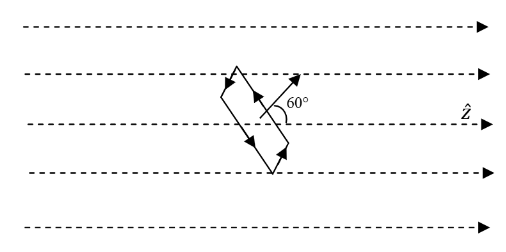
\includegraphics[width=0.6\textwidth]{figs/q44fig13.png}
\caption{square loop in a magnetic field}
\label{fig:q44}
\end{figure}

\item A spin-half particle is in a linear superposition $0.8|\uparrow\rangle + 0.6|\downarrow\rangle$ of its spin-up and spin-down states. If $|\uparrow\rangle$ and $|\downarrow\rangle$ are the eigenstates of $\sigma_z$ then what is the expectation value, up to one decimal place, of the operator $10\sigma_z + 5\sigma_x$? Here, symbols have their usual meanings. \underline{\hspace{5em}}.
\hfill \textbf{(GATE PH 2013)}

\item Consider the wave function $A e^{ikr} (r_0/r)$, where $A$ is the normalization constant. For $r = 2r_0$, the magnitude of probability current density up to two decimal places, in units of $(A^2\hbar k/m)$, is \underline{\hspace{5em}}.
\hfill \textbf{(GATE PH 2013)}

\item An $n$-channel junction field effect transistor has $5\,\text{mA}$ source to drain current at shorted gate ($I_{\text{DSS}}$) and $5\,\text{V}$ pinch off voltage ($V_P$). Calculate the drain current in $\text{mA}$ for a gate-source voltage ($V_{\text{GS}}$) of $-2.5\,\text{V}$. The answer should be up to two decimal places. \underline{\hspace{5em}}.
\hfill \textbf{(GATE PH 2013)}

\textbf{Common Data Questions}

\textbf{Common Data for Questions 48 and 49:} There are four energy levels $E, 2E, 3E$ and $4E$ (where $E>0$). The canonical partition function of two particles is, if these particles are

\item two identical fermions
\begin{enumerate}
\item $e^{-2\beta E} + e^{-4\beta E} + e^{-6\beta E} + e^{-8\beta E}$
\item $e^{-3\beta E} + e^{-4\beta E} + 2e^{-5\beta E} + e^{-6\beta E} + e^{-7\beta E}$
\item $(e^{-\beta E} + e^{-2\beta E} + e^{-3\beta E} + e^{-4\beta E})^2$
\item $e^{-2\beta E} - e^{-4\beta E} + e^{-6\beta E} - e^{-8\beta E}$
\end{enumerate}

\item two distinguishable particles
\begin{enumerate}
\item $e^{-2\beta E} + e^{-4\beta E} + e^{-6\beta E} + e^{-8\beta E}$
\item $e^{-3\beta E} + e^{-4\beta E} + 2e^{-5\beta E} + e^{-6\beta E} + e^{-7\beta E}$
\item $(e^{-\beta E} + e^{-2\beta E} + e^{-3\beta E} + e^{-4\beta E})^2$
\item $e^{-2\beta E} - e^{-4\beta E} + e^{-6\beta E} - e^{-8\beta E}$
\end{enumerate}

\textbf{Common Data for Questions 50 and 51:} To the given unperturbed Hamiltonian
\begin{align*}
\myvec{5 & 2 & 0 \\ 2 & 5 & 0 \\ 0 & 0 & 2}
\end{align*}
we add a small perturbation given by
\begin{align*}
\varepsilon \myvec{1 & 1 & 1 \\ 1 & 1 & -1 \\ 1 & -1 & 1}
\end{align*}
where $\varepsilon$ is a small quantity.

\item The ground state eigenvector of the unperturbed Hamiltonian is
\begin{enumerate}
\begin{multicols}{2}
\item $\left(1/\sqrt{2}, 1/\sqrt{2}, 0\right)$
\item $\left(1/\sqrt{2}, -1/\sqrt{2}, 0\right)$
\item $(0,0,1)$
\item $(1,0,0)$
\end{multicols}
\end{enumerate}

\item A pair of eigenvalues of the perturbed Hamiltonian, using first order perturbation theory, is
\begin{enumerate}
\begin{multicols}{4}
\item $3+2\varepsilon, 7+2\varepsilon$
\item $3+2\varepsilon, 2+\varepsilon$
\item $3, 7+2\varepsilon$
\item $3, 2+\varepsilon$
\end{multicols}
\end{enumerate}

\textbf{Linked Answer Questions}

\textbf{Statement for Linked Answer Questions 52 and 53:} In the Schmidt model of nuclear magnetic moments, we have,
\begin{align*}
 \vec{\mu} = \frac{e\hbar}{2Mc}(g_l \vec{l} + g_s \vec{s})
\end{align*}
where the symbols have their usual meaning.

\item For the case $J = l + 1/2$, where $J$ is the total angular momentum, the expectation value of $\vec{s} \cdot \vec{J}$ in the nuclear ground state is equal to,
    \begin{multicols}{4}
        \begin{enumerate}
            \item $(J-1)/2$
            \item $(J+1)/2$
            \item $J/2$
            \item $-J/2$
        \end{enumerate}
    \end{multicols}
    \hfill \textbf{(GATE PH 2013)}

\item For the $\text{O}^{17}$ nucleus (A=17, Z=8), the effective magnetic moment is given by, $\vec{\mu}_{eff} = \frac{e\hbar}{2Mc} g \vec{J}$, where $g$ is equal to, ($g_s = 5.59$ for proton and $-3.83$ for neutron)
    \begin{multicols}{4}
        \begin{enumerate}
            \item $1.12$
            \item $-0.77$
            \item $-1.28$
            \item $1.28$
        \end{enumerate}
    \end{multicols}
    \hfill \textbf{(GATE PH 2013)}

\textbf{Statement for Linked Answer Questions 54 and 55:} Consider the following circuit
\begin{figure}[H]
\centering
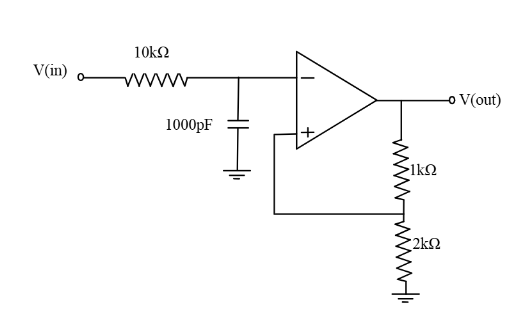
\includegraphics[width=0.5\textwidth]{figs/q54fig13.png}
\caption{Circuit diagram}
\label{fig:q54_55}
\end{figure}

\item For this circuit the frequency above which the gain will decrease by 20 $dB$ per decade is
\begin{enumerate}
\begin{multicols}{4}
\item 15.9 kHz
\item 1.2 kHz
\item 5.6 kHz
\item 22.5 kHz
\end{multicols}
\end{enumerate}

\item At 1.2kHz the closed loop gain is
\begin{enumerate}
\begin{multicols}{4}
\item 1
\item 1.5
\item 3
\item 0.5
\end{multicols}
\end{enumerate}

\textbf{Q. 56 -- Q. 60 carry one mark each.}

\begin{enumerate}[label=\textbf{Q.\arabic*}, start=56]

\item A number is as much greater than 75 as it is smaller than 117. The number is:
    \begin{multicols}{4}
        \begin{enumerate}
            \item 91
            \item 93
            \item 89
            \item 96
        \end{enumerate}
    \end{multicols}

\item Which of the following underlined parts of the sentence is grammatically incorrect?
\begin{align*}
\underset{\text{I}} {\underline{\text{The professor }}}\text{ } \underset{\text{II}}{\underline{\text{ordered to}}}\text{ } \underset{\text{III}}{\underline{\text{the students to go}}}\text{ } \underset{\text{IV}}{\underline{\text{out of the class}}}.
\end{align*}
    \begin{multicols}{4}
        \begin{enumerate}
            \item I
            \item II
            \item III
            \item IV
        \end{enumerate}
    \end{multicols}

\item Which of the following options is the closest in meaning to the word given below:
\begin{quote}
        Primeval
\end{quote}
    \begin{multicols}{2}
        \begin{enumerate}
            \item Modern
            \item Historic
            \item Primitive
            \item Antique
        \end{enumerate}
    \end{multicols}

\item Friendship, no matter how \underline{\hspace{8em}} it is, has its limitations.
    \begin{enumerate}
        \item cordial
        \item intimate
        \item secret
        \item pleasant
    \end{enumerate}

\item Select the pair that best expresses a relationship similar to that expressed in the pair:
    \begin{center}
        \textbf{Medicine: Health}
    \end{center}
    \begin{multicols}{2}
        \begin{enumerate}
            \item Science: Experiment
            \item Wealth: Peace
            \item Education: Knowledge
            \item Money: Happiness
        \end{enumerate}
    \end{multicols}
\end{enumerate}

\textbf{Q. 61 to Q. 65 carry two marks each.}

\begin{enumerate}[label=\textbf{Q.\arabic*}, start=61]

    \item X and Y are two positive real numbers such that $2X + Y \le 6$ and $X + 2Y \le 8$. For which of the following values of $(X,Y)$ the function $f(X,Y) = 3X + 6Y$ will give maximum value?
    \begin{enumerate}
        \item $(4/3, 10/3)$
        \item $(8/3, 20/3)$
        \item $(8/3, 10/3)$
        \item $(4/3, 20/3)$
    \end{enumerate}

    \item If $|4X - 7| = 5$ then the values of $2|X| - |-X|$ is:
    \begin{multicols}{4}
        \begin{enumerate}
            \item $2, 1/3$
            \item $1/2, 3$
            \item $3/2, 9$
            \item $2/3, 9$
        \end{enumerate}
    \end{multicols}

\item Following table provides figures (in rupees) on annual expenditure of a firm for two years - 2010 and 2011.
\begin{center}
\begin{tabular}{|l|c|c|}
\hline
\textbf{Category} & \textbf{2010} & \textbf{2011} \\
\hline
Raw material & 5200 & 6240 \\
\hline
Power \& fuel & 7000 & 9450 \\
\hline
Salary \& wages & 9000 & 12600 \\
\hline
Plant \& machinery & 20000 & 25000 \\
\hline
Advertising & 15000 & 19500 \\
\hline
Research \& Development & 22000 & 26400 \\
\hline
\end{tabular}
\end{center}
In 2011, which of the following two categories have registered increase by same percentage?
\begin{enumerate}
\item Raw material and Salary \& wages
\item Salary \& wages and Advertising
\item Power \& fuel and Advertising
\item Raw material and Research \& Development
\end{enumerate}

\item A firm is selling its product at Rs. 60 per unit. The total cost of production is Rs. 100 and firm is earning total profit of Rs. 500. Later, the total cost increased by 30\%. By what percentage the price should be increased to maintained the same profit level.
    \begin{multicols}{4}
        \begin{enumerate}
            \item 5
            \item 10
            \item 15
            \item 30
        \end{enumerate}
    \end{multicols}

    \item Abhishek is elder to Savar. \\
    Savar is younger to Anshul.
    \vspace{4mm}

    Which of the given conclusions is logically valid and is inferred from the above statements?
    \begin{enumerate}
        \item Abhishek is elder to Anshul
        \item Anshul is elder to Abhishek
        \item Abhishek and Anshul are of the same age
        \item No conclusion follows
    \end{enumerate}

\end{enumerate}

\vspace{5mm}

\begin{center}
    \textbf{END OF THE QUESTION PAPER}
\end{center}

\end{enumerate}

\end{document}